
%(BEGIN_QUESTION)
% Copyright 2012, Tony R. Kuphaldt, released under the Creative Commons Attribution License (v 1.0)
% This means you may do almost anything with this work of mine, so long as you give me proper credit

\centerline{\bf Reglene i \underbar{Fault Club}}

\begin{itemize}
\item{$(1)$} Ikke prøv å finne feilen ved å lete etter den -- utfør diagnostiske tester i stedet
\vskip 10pt
\item{$(2)$} {\it Ikke prøv å finne feilen ved å lete etter den -- utfør diagnostiske tester i stedet!}
\vskip 10pt
\item{$(3)$} Feilsøkingen er over når du korrekt har identifisert både typen feil og hvor den sitter
\vskip 10pt
\item{$(4)$} Det er bare deg og feilen -- ikke be om hjelp før du har brukt opp egne ressurser
\vskip 10pt
\item{$(5)$} Anta én feil om gangen, med mindre data viser noe annet
\vskip 10pt
\item{$(6)$} Ingen nye komponenter tillatt -- å bytte mistenkte dårlige komponenter med nye er sløsing med tid og penger
\vskip 10pt
\item{$(7)$} Vi øver så mange ganger som nødvendig til du mestrer dette
\vskip 10pt
\item{$(8)$} Feilsøking er ikke tilskuersport: \underbar{\it du} må feilsøke!
\end{itemize}

\vskip 10pt

Disse reglene vil garantert hjelpe deg å bli en bedre feilsøker, og de vil bli konsekvent understreket av instruktøren.


\filbreak

\noindent
{\bf Mal for sløyfediagram}

$$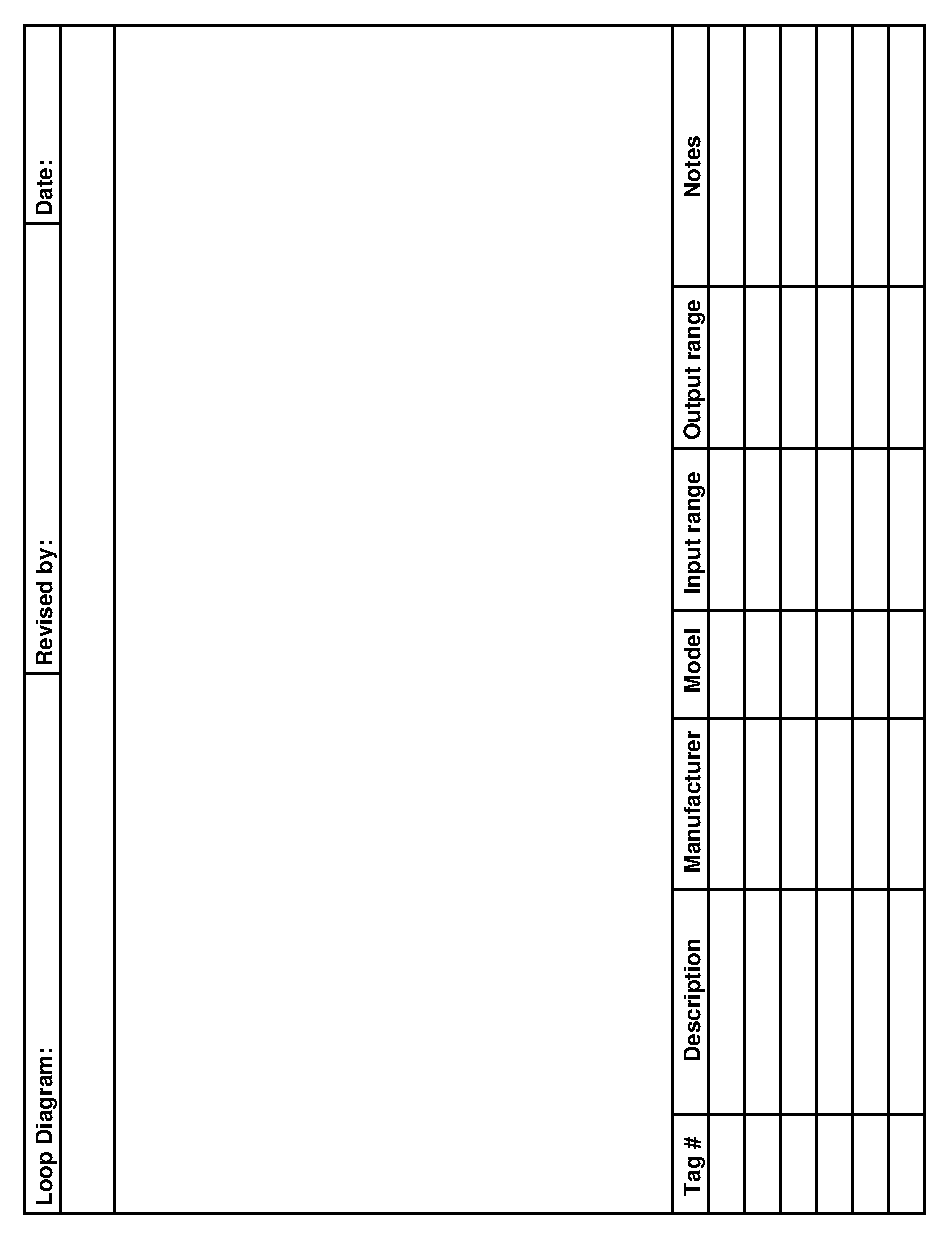
\includegraphics[width=15.5cm]{i00654x01.eps}$$

\vfil \eject

\noindent
{\bf Krav til sløyfediagram}

Den kanskje viktigste regelen når du lager et sløyfediagram er at {\it diagrammet skal være komplett og detaljert nok til at selv noen som ikke er instrumenttekniker kan forstå hvor hver ledning og hvert rør skal kobles i systemet!}

\begin{itemize}
\item{} {\bf Instrumentbobler}
\item{} Korrekte symboler og betegnelser brukt for alle instrumenter.
\item{} Alle instrumentbobler tydelig merket (bokstavkoder og sløyfenummer).
\item{} Alle instrumentbobler merket med riktige linjer (heltrukket, stiplet, enkel linje, dobbel linje, ingen linjer).
\item{} {\it Valgfritt:} Kalibreringsområder og virkningspiler skrevet ved hver boble.
\end{itemize}

\begin{itemize}
\item{} {\bf Tekstbeskrivelser}
\item{} Hvert instrument dokumentert under diagrammet (tagnummer, beskrivelse osv.).
\item{} Kalibrering (inngangs- og utgangsområde) oppgitt for hvert instrument, der det er relevant.
\end{itemize}

\begin{itemize}
\item{} {\bf Tilkoblingspunkter}
\item{} Alle terminaler og rørforgreninger tydelig merket.
\item{} Alle rekkeklemmer tydelig merket.
\item{} Alle koblingsbokser ("felt") vist som egne seksjoner i sløyfediagrammet, og tydelig merket.
\item{} Alle kontrollpanel vist som egne seksjoner i sløyfediagrammet, og tydelig merket.
\item{} Alle lederfarger vist ved hver terminal.
\item{} Alle terminaler på instrumenter merket slik de fremstår på instrumentet (slik at leseren vet nøyaktig hvilken instrumentterminal hver leder går til).
\end{itemize}

\begin{itemize}
\item{} {\bf Kabler og rør}
\item{} Enkeltpar-kabler eller pneumatiske rør til enkeltinstrumenter bør merkes med feltinstrumentets tagnummer (f.eks. "TT-8" eller "TY-12").
\item{} Flerpar-kabler eller rørbunter mellom koblingsbokser og/eller paneler må ha unike nummer (f.eks. "Kabel 10") samt nummer for hvert par (f.eks. "Par 1", "Par 2" osv.).
\end{itemize}

\begin{itemize}
\item{} {\bf Energikilder}
\item{} Alle forsyningsnivåer merket (f.eks. "24 VDC", "120 VAC", "20 PSI").
\item{} Alle avstengningspunkter merket (f.eks. "Sikring \#5", "Ventil \#7").
\end{itemize}

\vfil \eject

\noindent
{\bf Eksempel på sløyfediagram (med enkelt-sløyfe regulator)}

$$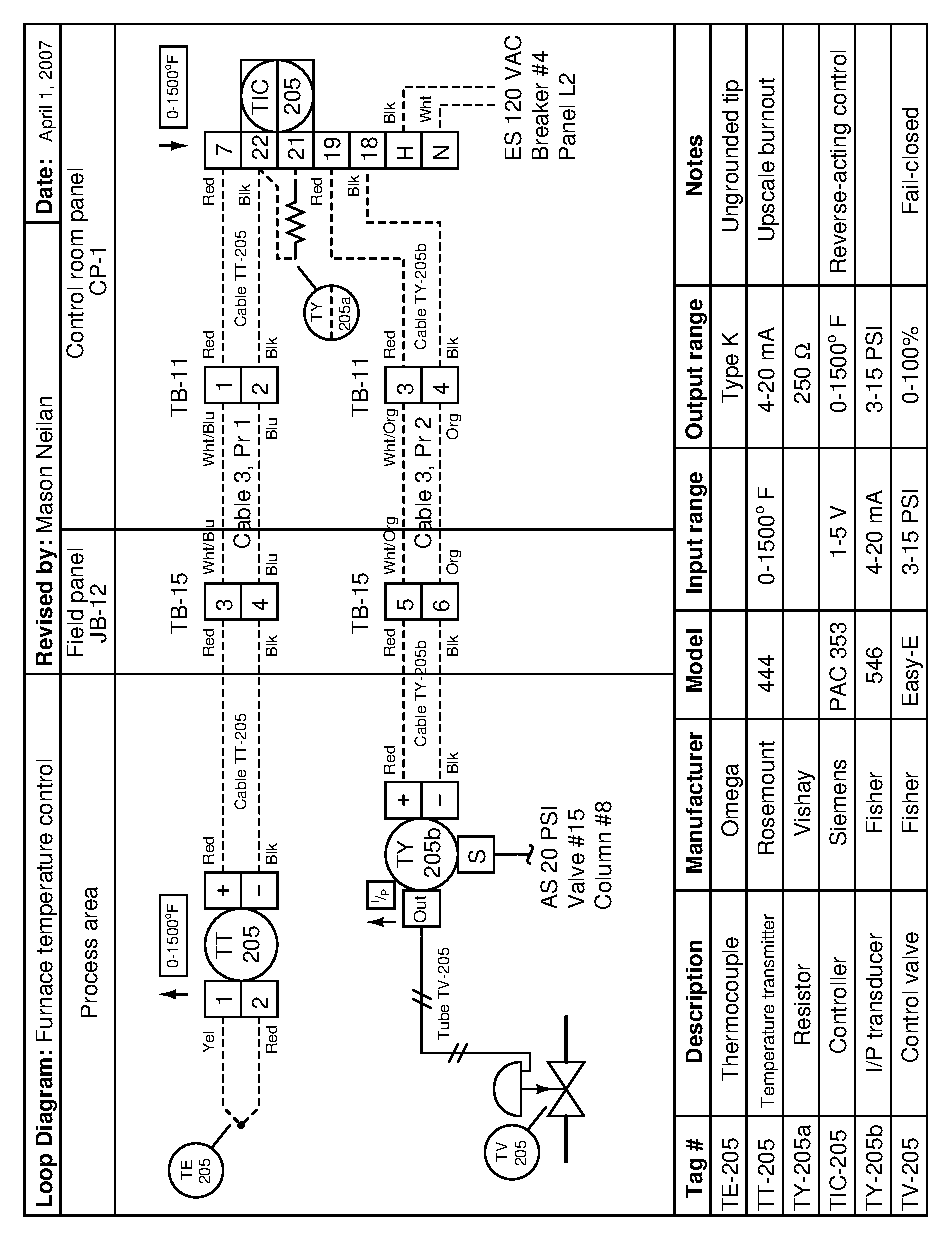
\includegraphics[width=15.5cm]{i00654x02.eps}$$


\vfil \eject

\noindent
{\bf Eksempel på sløyfediagram (med DCS-regulator)}

$$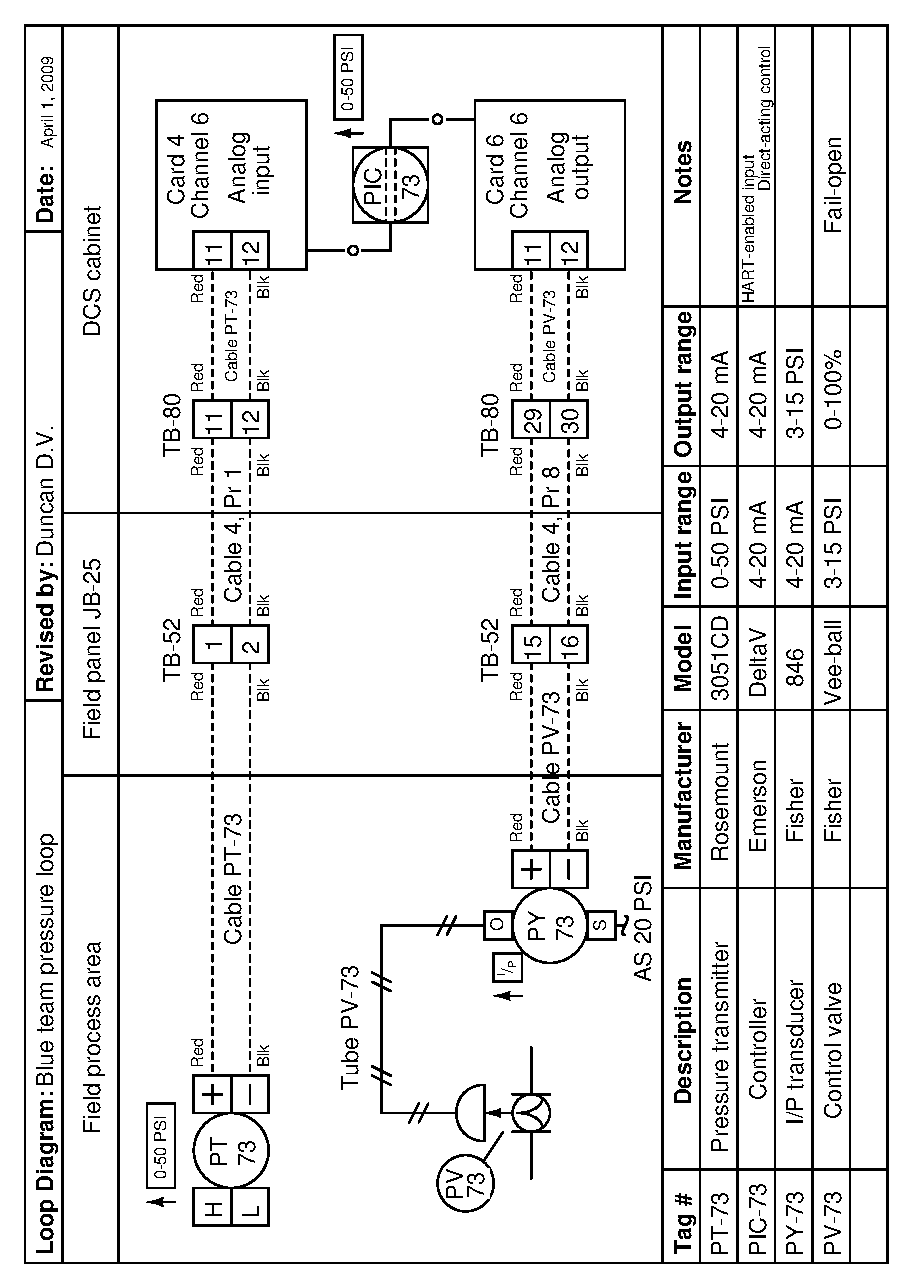
\includegraphics[width=15.5cm]{i00654x03.eps}$$


\vfil \eject

\noindent
{\bf Eksempel på sløyfediagram (med pneumatisk regulator)}

$$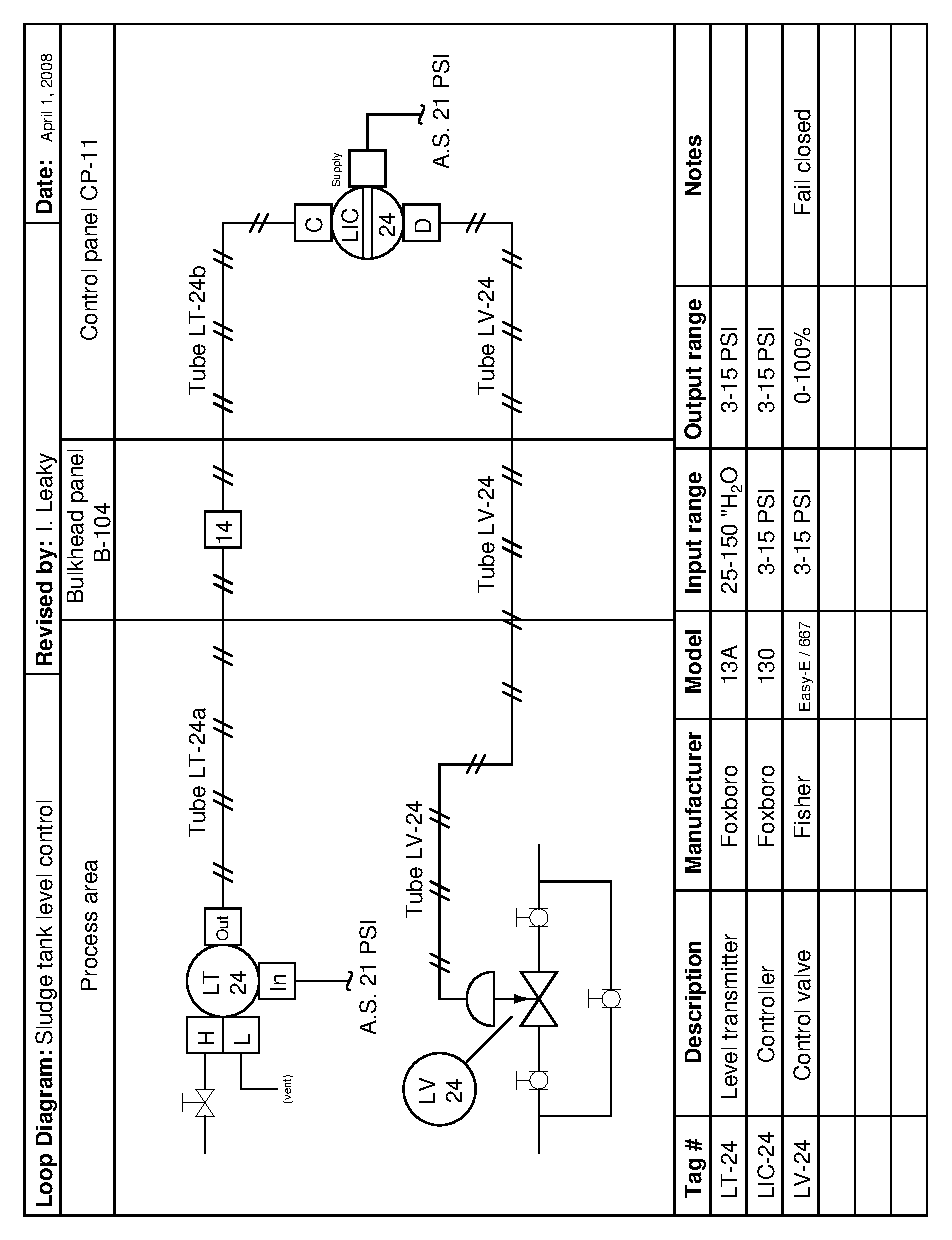
\includegraphics[width=15.5cm]{i00654x04.eps}$$


\vfil \eject

\noindent
{\bf Eksempel på sløyfediagram (med PLC, med elektronisk posisjoner montert på ventil)}

$$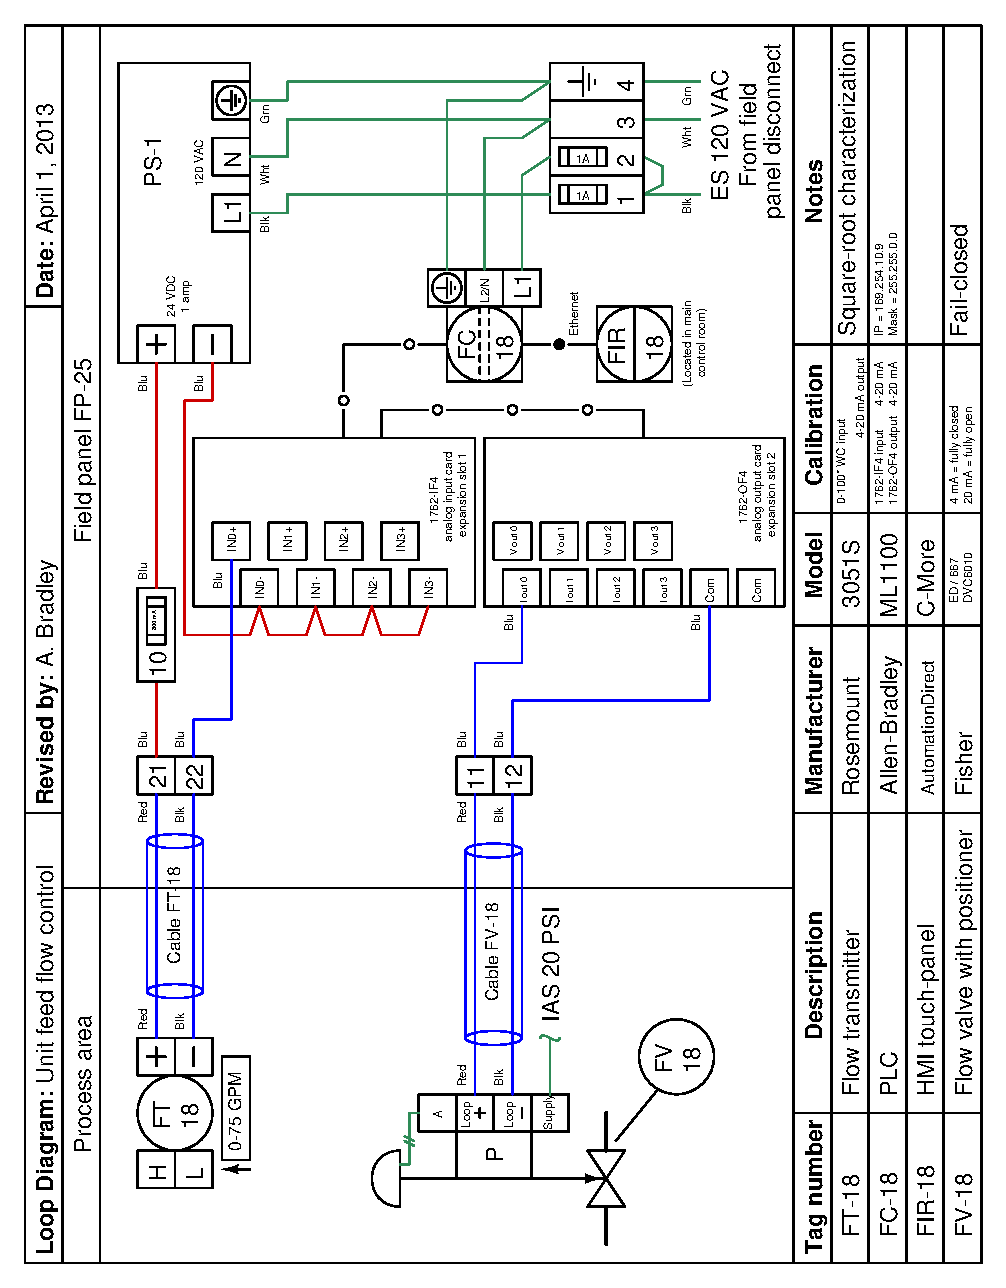
\includegraphics[width=15.5cm]{i00654x05.eps}$$

\underbar{file i00654no}
%(END_QUESTION)





%(BEGIN_ANSWER)

Sløyfediagrammet ditt blir godkjent når instruktøren inspiserer sløyfen sammen med deg og resten av teamet.

%(END_ANSWER)





%(BEGIN_NOTES)


%INDEX% Labøvelse, mal og krav for sløyfediagram

%(END_NOTES)
